\chapter{Portable Executable Format} \label{chap:peformat}

The \PE{} is a file format for executables and object files used by Microsoft products. Some examples for \PE{} file types are \DLL{}, \FON{}, \DRV{}, \SYS{} and \EXE{} files.

PortEx extracts the information from the \PE{} format to assist in analysing malware. Therefore knowledge about the \PE{} format is neccessary to understand the inner workings of the library PortEx.

The \PE{} format is described in the \emph{Microsoft Portable Executable and Common Object File Format Specification} \cite{pespec}

\section{General Structure}

Figure~\ref{fig:peformat} illustrates the structure of a \PE{} file. An executable \PE{} file always starts with the MS-DOS Stub. This is an application which is able to run in MS-DOS. It prints the message \enquote{This program cannot be run in DOS mode}. The offset to the \PE{} signature is in location 0x3c of the stub and enables Windows to properly execute the \PE{} file. Right after the signature follow the COFF File Header, the Optional Header and the Section Table.

The Section Table describes \ia{} characteristics, size and location of the sections that make up the rest of the \PE{} file.

\todo{make your own picture}
\begin{figure}
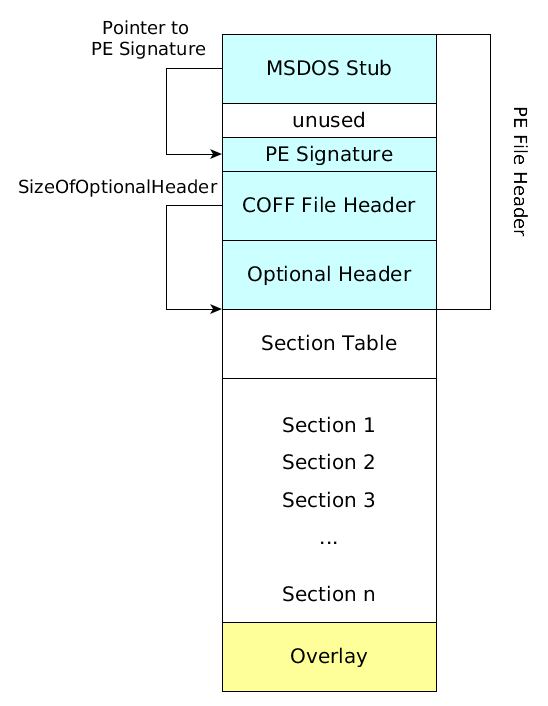
\includegraphics[width=.98\textwidth, height=\textheight,keepaspectratio]{graphics/peformat}
\caption{Structure of a PE file \protect{\cite{kath13}}}
\label{fig:peformat} 
\end{figure}

\section{Special Sections}

Sections may contain arbitrary information, which is only relevant to the application using them; but some sections have a special meaning. These sections can be recognized by certain flags that are set in the Section Table or by entries in the Data Directory Table of the Optional Header. The special sections also have typical section names, but their names are only a convention. They can not be relied on while trying to find certain sections.

Some of these special sections are described right after.

\subsection*{Import Section}

\subsection*{Resource Section}

\subsection*{Debug Section}
